% =============================================================
%  CS102-F26 Digital Design and Computer Architecture I
%  Lecture 12 -- Flip-Flops (Unit 12)
%  Follows Sections 5.3.3, 5.3.4 and 5.3.5 of
%  A Student's Computer Architecture Book I.
%
%  Build the slides and the print handout:  npm run materials -- lecture-12
% =============================================================
\makeatletter
\def\input@path{{templates/latex/}{../}}
\makeatother

\documentclass[10pt]{wosm-slides}
\usepackage{cs102-lectures}[2026/10/20]

\title[Lecture 12 \textperiodcentered\ Flip-Flops]{Flip-Flops}
\subtitle{Lecture 12: edge-triggered memory: D, T and JK flip-flops}

% ---------- Helpers for this lecture --------------------------
% Rising clock edges of the 16-step diagrams below.
\newcommand*\clockedges[1]{\foreach \t in {2,6,10,14} {\timingedge{\t}{#1}}}

% =============================================================
\begin{document}

\maketitle

\begin{frame}{Today}
  \tableofcontents
\end{frame}

% =============================================================
\section{Edges instead of levels}

\begin{frame}{Latches and flip-flops}
  \begin{columns}[c, totalwidth=\textwidth]
    \column{0.62\textwidth}
      \begin{itemize}
        \item A latch reacts to a \alert{level}: while $E = 1$ it is transparent.
          That is what went wrong at the end of Lecture 11.
        \item A \alert{flip-flop} reacts to an \alert{edge}: the instant the clock goes
          from 0 to 1 (or from 1 to 0).
      \end{itemize}
      \begin{definition}[D flip-flop]
        A rising-edge \emph{D flip-flop} stores the value of $D$ at each rising edge
        of the clock, and keeps it until the next one.
      \end{definition}
    \column{0.32\textwidth}
      \centering
      \begin{tikzpicture}[scale=1.4]
        \pic (f) at (0,0) {dff};
        \draw[wire] (f-d) -- ++(-0.4,0) node[left] {$D$};
        \draw[wire] (f-clk) -- ++(-0.4,0) node[left] {clk};
        \draw[wire] (f-q) -- ++(0.4,0) node[right] {$Q$};
      \end{tikzpicture}\par\medskip
      \wosmlabel{The triangle marks an edge-triggered clock input.}
  \end{columns}
\end{frame}

\begin{frame}{A latch and a flip-flop, side by side}
  \begin{center}
    \begin{tikzpicture}[x=0.62cm]
      \clockedges{4}
      \timingwave{0}{clk}{0,0,1,1,0,0,1,1,0,0,1,1,0,0,1,1}
      \timingwave{1}{$D$}{0,1,1,0,0,0,0,1,1,1,0,0,1,0,0,0}
      \timingwave{2}{latch $Q$}{0,0,1,0,0,0,0,1,1,1,0,0,0,0,0,0}
      \timingwave{3}{flip-flop $Q$}{0,0,1,1,1,1,0,0,0,0,1,1,1,1,0,0}
    \end{tikzpicture}
  \end{center}

  \begin{itemize}
    \item The latch, enabled by the clock, follows every change of $D$ while the clock
      is 1.
    \item The flip-flop changes only at the rising edges (the grey lines), to the
      value $D$ had just before the edge, and holds it for a whole period.
  \end{itemize}
\end{frame}

% =============================================================
\section{The master--slave D flip-flop}

\begin{frame}{Two latches make a flip-flop}
  \begin{center}
    \begin{tikzpicture}[gates]
      \pic (m) at (2,0) {dlatch};
      \pic (s) at (4.6,0) {dlatch};
      \node[above, font=\scriptsize] at (2,0.55) {master};
      \node[above, font=\scriptsize] at (4.6,0.55) {slave};
      \node[not gate] (n) at (0.7,-0.27) {};
      \draw[wire] (m-d) -- ++(-1.7,0) node[left] {$D$};
      \draw[wire] (n.output) -- (m-e);
      \draw[wire] (m-q) -- ++(0.5,0) |- (s-d);
      \draw[wire] (s-q) -- ++(0.5,0) node[right] {$Q$};
      \draw[wire] (n.input) -- ++(-0.3,0) coordinate (c) -- ++(0,-0.6) coordinate (c2);
      \draw[wire] (c2) -- ++(-0.4,0) node[left] {clk};
      \draw[wire] (c2) -| ($(s-e)+(-0.4,0)$) -- (s-e);
      \fill[wosm-text] (c2) circle (1.5pt);
      \node[edgelabel, above] at ($(m-q)+(0.3,0)$) {$Q_m$};
    \end{tikzpicture}
  \end{center}

  \begin{itemize}
    \item The \alert{master} latch is enabled by $\mathrm{clk}'$: it is transparent while
      the clock is 0.
    \item The \alert{slave} latch is enabled by clk: it is transparent while the clock
      is 1.
    \item The two are never transparent at the same time, so $D$ never runs straight
      through to $Q$.
  \end{itemize}
\end{frame}

\begin{frame}{How it works}
  \begin{columns}[c, totalwidth=\textwidth]
    \column{0.55\textwidth}
      \centering
      \begin{tikzpicture}[x=0.42cm]
        \clockedges{4}
        \timingwave{0}{clk}{0,0,1,1,0,0,1,1,0,0,1,1,0,0,1,1}
        \timingwave{1}{$D$}{0,1,1,0,0,0,0,1,1,1,0,0,1,0,0,0}
        \timingwave{2}{$Q_m$}{0,1,1,1,0,0,0,0,1,1,1,1,1,0,0,0}
        \timingwave{3}{$Q$}{0,0,1,1,1,1,0,0,0,0,1,1,1,1,0,0}
      \end{tikzpicture}
    \column{0.41\textwidth}
      \small
      \begin{itemize}
        \item Clock 0: the master follows $D$; the slave holds $Q$.
        \item Rising edge: the master closes on the last value of $D$; the slave opens
          and passes it to $Q$.
        \item Clock 1: $D$ may change, but the master is closed.
        \item Falling edge: the slave closes; the master opens again.
      \end{itemize}
  \end{columns}

  \bigskip
  Together: $Q$ takes the value of $D$ at each rising edge. In one line,
  $Q^{+} = D$.
\end{frame}

% =============================================================
\section{Reset}

\begin{frame}{A known starting state}
  \begin{itemize}
    \item When a circuit is switched on, its flip-flops hold random values. A
      \alert{reset} input puts them in a known state, $Q = 0$.
    \item \emph{Synchronous} reset: takes effect at the next clock edge. Just feed
      $D \cdot R'$ into the flip-flop.
    \item \emph{Asynchronous} reset: takes effect at once, whatever the clock is
      doing.
  \end{itemize}

  \medskip
  \begin{columns}[c, totalwidth=\textwidth]
    \column{0.4\textwidth}
      \centering
      \small
      \begin{tabular}{@{}ccc|c@{}}
        $R$ & clk & $D$ & $Q$ \\
        \midrule
        0 & 0 & $d$ & holds \\
        0 & $\uparrow$ & $d$ & $d$ \\
        0 & 1 & $d$ & holds \\
        0 & $\downarrow$ & $d$ & holds \\
        1 & any & any & 0 \\
      \end{tabular}
    \column{0.56\textwidth}
      \small
      The book's asynchronous reset adds a few gates in front of both latches:
      \begin{itemize}
        \item master: data $D \cdot R'$, enable $\mathrm{clk}' + R$;
        \item slave: data $Q_m \cdot R'$, enable $\mathrm{clk} + R$.
      \end{itemize}
      With $R = 1$ both latches are open and both receive 0: $Q = 0$ at once.
  \end{columns}
\end{frame}

\begin{frame}{Asynchronous reset in time}
  \begin{center}
    \begin{tikzpicture}[x=0.62cm]
      \clockedges{4}
      \timingwave{0}{clk}{0,0,1,1,0,0,1,1,0,0,1,1,0,0,1,1}
      \timingwave{1}{$D$}{1,1,1,1,1,1,1,1,0,0,0,0,1,1,1,1}
      \timingwave{2}{$R$}{0,0,0,0,0,1,1,0,0,0,0,0,0,0,0,0}
      \timingwave{3}{$Q$}{0,0,1,1,1,0,0,0,0,0,0,0,0,0,1,1}
    \end{tikzpicture}
  \end{center}

  \begin{itemize}
    \item $R$ rises between two edges, and $Q$ drops to 0 straight away.
    \item The edge at $t = 6$ comes while $R = 1$: it is ignored.
    \item After $R$ falls, the flip-flop works normally again: the edges at 10 and 14
      store 0 and 1.
  \end{itemize}
  \wosmlabel{The DX8's registers all have a reset input, so the whole computer starts
  from zero (Lecture 01's diagram).}
\end{frame}

% =============================================================
\section{T and JK flip-flops}

\begin{frame}{The T flip-flop}
  \begin{columns}[c, totalwidth=\textwidth]
    \column{0.5\textwidth}
      \centering
      \begin{tikzpicture}[gates]
        \pic (f) at (2.4,0) {dff};
        \pic (m) at (0.9,0.27) {mux};
        \node[not gate, scale=0.8] (n) at (-0.15,-0.03) {};
        \draw[wire] (m-out) -- (f-d);
        \draw[wire] (f-q) -- ++(0.4,0) coordinate (o) -- ++(0.4,0) node[right] {$Q$};
        \draw[wire] (o) |- (-0.85,1.2) |- (m-in0);
        \draw[wire] (-0.85,0.57) |- (n.input);
        \fill[wosm-text] (o) circle (1.5pt);
        \fill[wosm-text] (-0.85,0.57) circle (1.5pt);
        \draw[wire] (n.output) -- (m-in1);
        \draw[wire] (m-sel) -- ++(0,-0.5) -| (-1.1,-0.705) node[left] {$T$};
        \draw[wire] (f-clk) -- ++(-0.3,0) |- (-1.1,-1.15) node[left] {clk};
      \end{tikzpicture}
    \column{0.46\textwidth}
      \begin{tabular}{@{}c|c@{}}
        $T$ & $Q^{+}$ \\
        \midrule
        0 & $Q$ (hold) \\
        1 & $Q'$ (toggle) \\
      \end{tabular}\par\medskip
      $Q^{+} = T \oplus Q$, at each rising edge.\par\medskip
      Built as in the book: a D flip-flop, and a multiplexer that feeds it $Q$ or $Q'$.
  \end{columns}

  \bigskip
  \wosmlabel{Lecture 01's lamp with a push button is a T flip-flop, and each press
  toggles it.}
\end{frame}

\begin{frame}{Toggling halves the frequency}
  \begin{center}
    \begin{tikzpicture}[x=0.62cm]
      \foreach \t in {1,3,5,7,9,11,13,15} {\timingedge{\t}{2}}
      \timingwave{0}{clk}{0,1,0,1,0,1,0,1,0,1,0,1,0,1,0,1}
      \timingwave{1}{$Q$, $T = 1$}{0,1,1,0,0,1,1,0,0,1,1,0,0,1,1,0}
    \end{tikzpicture}
  \end{center}

  \begin{itemize}
    \item With $T = 1$, $Q$ flips at every rising edge: one period of $Q$ takes two
      clock periods.
    \item A 100\,MHz clock gives a 50\,MHz $Q$. Chain such flip-flops, and each one
      halves the frequency again: that is a counter \unitref{13}.
  \end{itemize}
\end{frame}

\begin{frame}{The JK flip-flop}
  \begin{columns}[c, totalwidth=\textwidth]
    \column{0.36\textwidth}
      \centering
      \begin{tabular}{@{}cc|c@{}}
        $J$ & $K$ & $Q^{+}$ \\
        \midrule
        0 & 0 & $Q$ (hold) \\
        0 & 1 & 0 (reset) \\
        1 & 0 & 1 (set) \\
        1 & 1 & $Q'$ (toggle) \\
      \end{tabular}\par\medskip
      \wosmlabel{at each rising edge; between edges, $Q$ holds}
    \column{0.6\textwidth}
      \begin{itemize}
        \item Like an SR latch with $J$ for set and $K$ for reset, but $J = K = 1$ is
          allowed: it toggles.
        \item As an equation: $Q^{+} = J Q' + K' Q$.
        \item Built as in the book: a D flip-flop fed by a 4-to-1 multiplexer with
          select $JK$ and data $Q$, 0, 1, $Q'$.
      \end{itemize}
  \end{columns}

  \begin{center}
    \begin{tikzpicture}[gates]
      \pic (m) at (0,0) {mux4};
      \pic (f) at (1.8,-0.27) {dff};
      \foreach \i/\x in {0/Q, 1/0, 2/1, 3/Q'}
        \draw[wire] (m-in\i) -- ++(-0.4,0) node[left, font=\scriptsize] {$\x$};
      \draw[wire] (m-out) -- (f-d);
      \draw[wire] (m-sel) -- ++(0,-0.3) node[below, font=\scriptsize] {$J K$};
      \draw[wire] (f-clk) -- ++(-0.25,0) -- ++(0,-0.71)
        node[below, font=\scriptsize] {clk};
      \draw[wire] (f-q) -- ++(0.4,0) node[right] {$Q$};
    \end{tikzpicture}
  \end{center}
\end{frame}

\begin{frame}{All of them}
  \begin{center}
    \begin{tabular}{@{}llll@{}}
      \toprule
      & Reacts to & Next value & Watch out \\
      \midrule
      SR latch & levels & $Q^{+} = S + R' Q$ & $S = R = 1$ not allowed \\
      D latch & the level of $E$ & $Q^{+} = D$ while $E = 1$ & transparent \\
      D flip-flop & clock edges & $Q^{+} = D$ & \\
      T flip-flop & clock edges & $Q^{+} = T \oplus Q$ & \\
      JK flip-flop & clock edges & $Q^{+} = J Q' + K' Q$ & \\
      \bottomrule
    \end{tabular}
  \end{center}

  \bigskip
  \begin{remark}
    The D flip-flop is enough to build the other two, as we just did. Most digital
    designs, including the DX8, use D flip-flops everywhere.
  \end{remark}
\end{frame}

% =============================================================
\section{Registers}

\begin{frame}{From one bit to a register}
  \begin{columns}[c, totalwidth=\textwidth]
    \column{0.42\textwidth}
      \centering
      \begin{tikzpicture}[gates]
        \foreach \i/\y in {0/1.65, 1/0.55, 2/-0.55, 3/-1.65} {
          \pic (f\i) at (0,\y) {dff};
          \draw[wire] (f\i-d) -- ++(-0.5,0) node[left, font=\scriptsize] {$D_{\i}$};
          \draw[wire] (f\i-q) -- ++(0.4,0) node[right, font=\scriptsize] {$Q_{\i}$};
          \draw[wire] (f\i-clk) -- ++(-0.2,0) coordinate (c\i);
        }
        \draw[wire] (c0) -- (c3) -- ++(0,-0.6) -- ++(-0.6,0) node[left, font=\scriptsize]
          {clk};
      \end{tikzpicture}
    \column{0.54\textwidth}
      \begin{itemize}
        \item $n$ D flip-flops that share one clock store an $n$-bit number: a
          \alert{register}. The book's 8-bit register is just 8 of them.
        \item To load only when told, put a 2-to-1 multiplexer in front of each $D$:
          it passes $Q_i$ (keep) or $D_i$ (load), chosen by a write-enable bit.
        \item The DX8's register file holds 8 such registers \unitref{19}.
      \end{itemize}
  \end{columns}
\end{frame}

\begin{frame}{Try it}
  \begin{enumerate}
    \item A D flip-flop starts with $Q = 0$. Just before four rising edges, $D$ is 1,
      0, 0, 1. What is $Q$ after each edge?\par
      \uncover<2->{\small 1, 0, 0, 1: it copies $D$ at each edge.}
    \item A T flip-flop with $T = 1$ runs on a 100\,MHz clock. What does its output
      look like?\par
      \uncover<3->{\small A 50\,MHz square wave: it flips once per clock period.}
    \item A JK flip-flop has $J = K = 1$ and starts at $Q = 0$. What is $Q$ after three
      rising edges?\par
      \uncover<4->{\small 1, then 0, then 1: it toggles each time.}
    \item Build a T flip-flop and a D flip-flop from a JK flip-flop.\par
      \uncover<5->{\small T: $J = K = T$. D: $J = D$, $K = D'$.}
  \end{enumerate}
\end{frame}

% =============================================================
\section{Summary}

\begin{frame}{Summary}
  \begin{itemize}
    \item A flip-flop changes only at a clock edge; a latch is transparent for as long
      as it is enabled.
    \item The master--slave D flip-flop: two D latches enabled by $\mathrm{clk}'$ and
      clk. $Q$ takes the value of $D$ at each rising edge.
    \item Reset puts a flip-flop in a known state: synchronously at the next edge, or
      asynchronously at once.
    \item T flip-flop: $Q^{+} = T \oplus Q$. JK flip-flop: $Q^{+} = J Q' + K' Q$. Both
      are a D flip-flop with a multiplexer in front.
    \item $n$ flip-flops sharing a clock form an $n$-bit register.
  \end{itemize}
\end{frame}

\begin{frame}{Before the next lecture}
  \begin{itemize}
    \item Read Sections~5.3.3, 5.3.4 and 5.3.5 of the book.
    \item In Logisim-evolution, build the master--slave D flip-flop from your D
      latches, add the asynchronous reset, and compare it with the D flip-flop in the
      Memory library.
    \item Build a T flip-flop from it, connect $T$ to 1, and watch $Q$ in a timing
      diagram.
  \end{itemize}

  \begin{block}{Next lecture \unitref{13}}
    Counters: the synchronous up counter and the asynchronous ripple counter.
  \end{block}
\end{frame}

\end{document}
